\documentclass{scrreprt}
\usepackage{listings}
\usepackage{underscore}
\usepackage[bookmarks=true]{hyperref}
\usepackage[utf8]{inputenc}
\usepackage[english]{babel}
\usepackage{graphicx}
\graphicspath{{work_packages/work_package_1/static/ui-design/}} % path relative to root
%\graphicspath{{static/ui-design/}}
\hypersetup{
    pdftitle={Software Requirement Specification},    % title
    pdfauthor={Training Montage},                     % author
    pdfsubject={TeX and LaTeX},                        % subject of the document
    pdfkeywords={TeX, LaTeX, graphics, images}, % list of keywords
    colorlinks=true,       % false: boxed links; true: colored links
    linkcolor=blue,       % color of internal links
    citecolor=black,       % color of links to bibliography
    filecolor=black,        % color of file links
    urlcolor=purple,        % color of external links
    linktoc=page            % only page is linked
}

\def\myversion{0.1 }
\date{}

\usepackage{hyperref}
\begin{document}

\begin{flushright}
    \rule{16cm}{5pt}\vskip1cm
    \begin{bfseries}
        \Huge{UI DESIGN}\\
        \vspace{.9cm}
        for\\
        \vspace{.9cm}
        COE 1186 Project\\
        \vspace{.9cm}
        \LARGE{Version \myversion approved}\\
        \vspace{.9cm}
        Prepared by:\\
        Alec Rosenbaum\\
        Aric Hudson\\
        Isaac Goss\\
        Mitch Moran\\
        Parth Dadhania\\
        \vspace{1.9cm}
        Training Montage\\
        \vspace{.9cm}
        \today\\
    \end{bfseries}
\end{flushright}

\tableofcontents


%%%%%%%%%%%%%%%%%%   CTC Start   %%%%%%%%%%%%%%%%%%%%%
\chapter{Centralized Traffic Control}

% picture(s) of overall gui
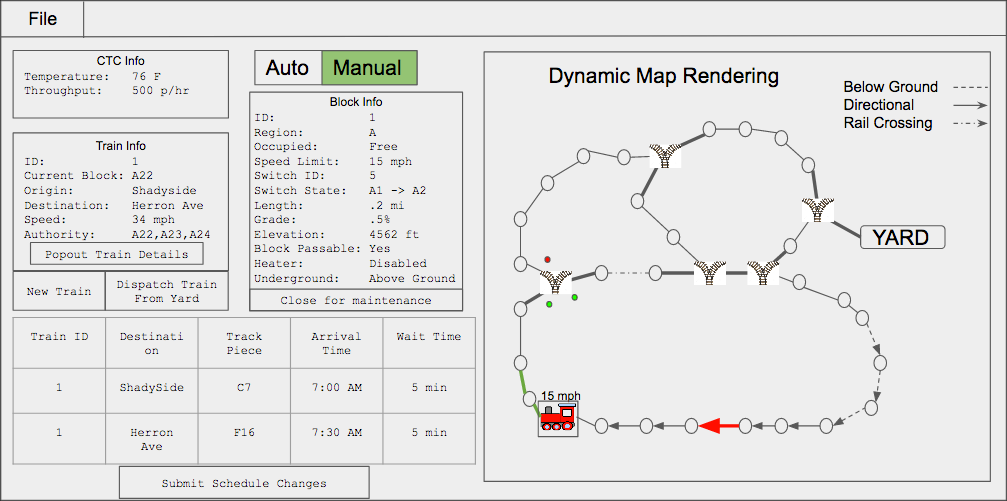
\includegraphics[width=\textwidth]{CTC-main}

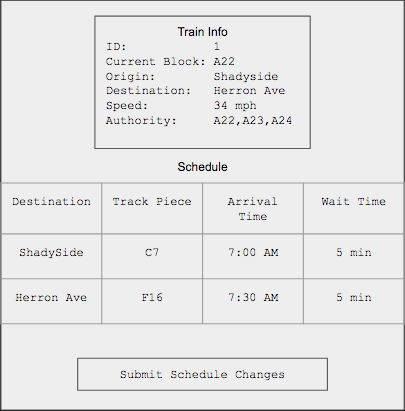
\includegraphics[width=\textwidth]{CTC-pop}

\chapter{Track Model}

% picture(s) of overall gui
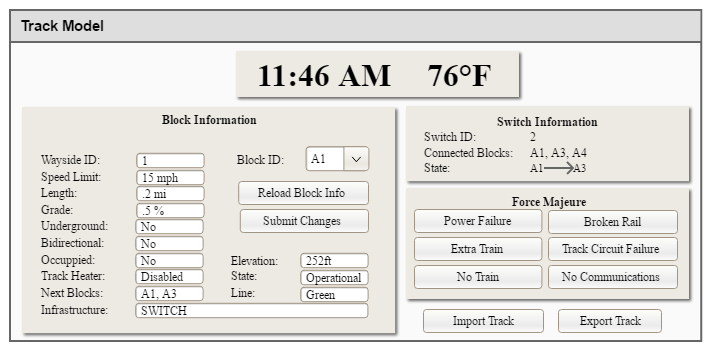
\includegraphics[width=\textwidth]{track-model}

\chapter{Wayside Controller}
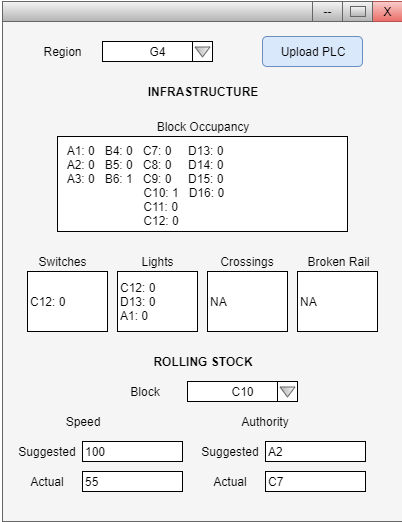
\includegraphics[width=\textwidth]{wc-ui}

\chapter{Train Model}
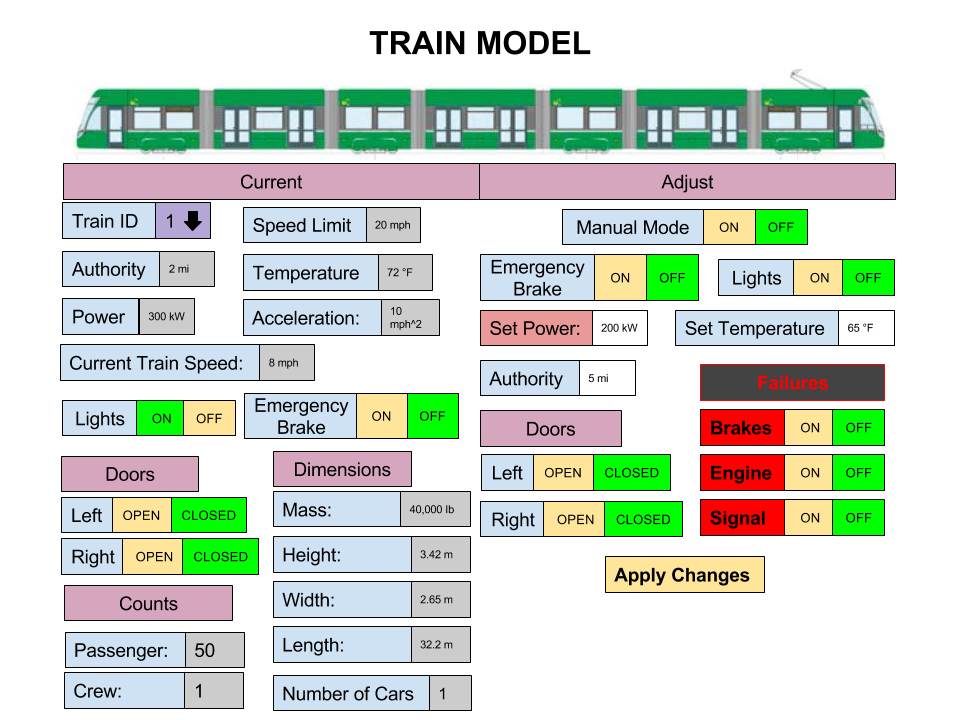
\includegraphics[width=\textwidth]{TrainModelUI}

\chapter{Train Controller}
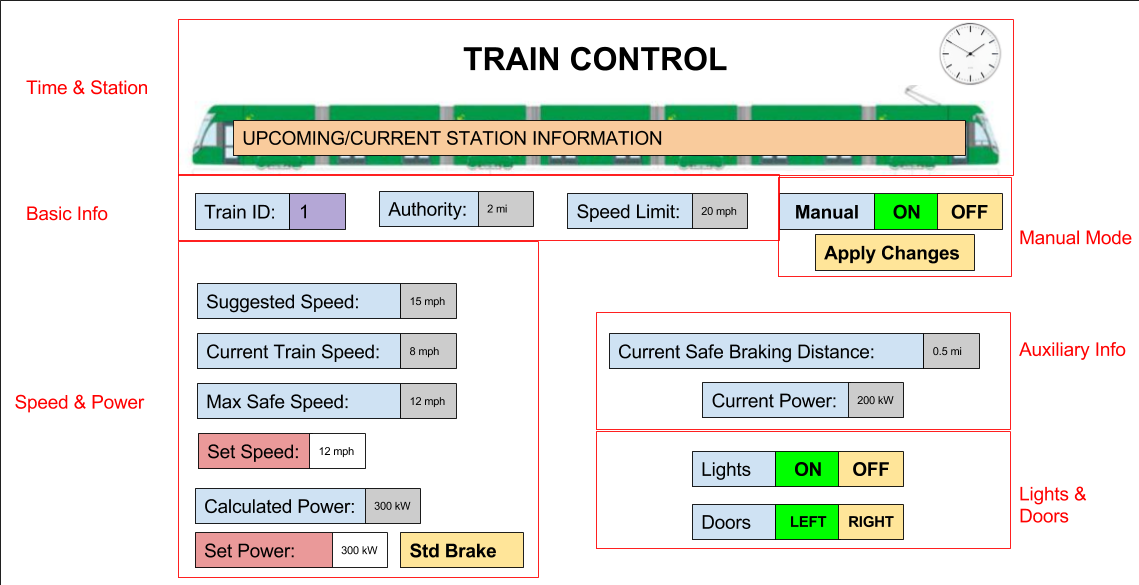
\includegraphics[width=\textwidth]{tc}
\end{document}
